%%%%%%%%%%%%%%%%%%%%%%%%%%%%%%%%%%%%%%%%%%%%%%%%%%%%%%%%%%%%%%%%%%%%%%%%%%%%%%%%%%
\begin{frame}[fragile]\frametitle{}
\begin{center}
{\Large LLM Evaluation}
\end{center}
\end{frame}

%%%%%%%%%%%%%%%%%%%%%%%%%%%%%%%%%%%%%%%%%%%%%%%%%%%%%%%%%%%
\begin{frame}[fragile]\frametitle{Overview}
  \begin{itemize}
    \item Evaluating LLM outputs is crucial for robust applications.
    \item LLM evaluation is challenging but necessary.
    \item Refining accuracy or enhancing RAG systems requires understanding LLM evaluation metrics.
  \end{itemize}

Importance of Metrics:
  \begin{itemize}
    \item Metrics are vital for a bulletproof LLM evaluation pipeline.
    \item Understanding common pitfalls is crucial.
    \item Great LLM metrics enhance model development.
  \end{itemize}
  
Scoring Methods:
  \begin{itemize}
    \item Various methods exist for scoring LLM metrics.
    \item Exploring different approaches is essential.
  \end{itemize}
\end{frame}

%%%%%%%%%%%%%%%%%%%%%%%%%%%%%%%%%%%%%%%%%%%%%%%%%%%%%%%%%%%
\begin{frame}[fragile]\frametitle{Evaluating Large Language Models (1)}
  \begin{itemize}
    \item \textbf{Understanding Needs:}
      \begin{itemize}
        \item Crucial to evaluate whether LLMs meet specific requirements.
      \end{itemize}
    \item \textbf{Clear Metrics:}
      \begin{itemize}
        \item Establish clear metrics to gauge the value added by LLM applications.
      \end{itemize}
    \item \textbf{Comprehensive Evaluation:}
      \begin{itemize}
        \item Encompasses assessing the entire pipeline, including prompts, retrieved documents, and processed content.
      \end{itemize}
  \end{itemize}
\end{frame}

%%%%%%%%%%%%%%%%%%%%%%%%%%%%%%%%%%%%%%%%%%%%%%%%%%%%%%%%%%%
\begin{frame}[fragile]\frametitle{Evaluating Large Language Models (2)}
  \begin{itemize}
    \item \textbf{Pipeline Evaluation:}
      \begin{itemize}
        \item Assess the effectiveness of individual components within the LLM pipeline.
        \item Includes evaluation of prompts and quality of retrieved documents.
      \end{itemize}
    \item \textbf{Model Evaluation:}
      \begin{itemize}
        \item Evaluate the performance of the LLM model itself.
        \item Focus on the quality and relevance of its generated output.
      \end{itemize}
  \end{itemize}
\end{frame}

%%%%%%%%%%%%%%%%%%%%%%%%%%%%%%%%%%%%%%%%%%%%%%%%%%%%%%%%%%%
\begin{frame}[fragile]\frametitle{Evaluating Large Language Models (3)}
  \begin{itemize}
    \item \textbf{Prompt Quality:}
      \begin{itemize}
        \item Assess the appropriateness and effectiveness of prompts used for LLMs.
      \end{itemize}
    \item \textbf{Document Retrieval Quality:}
      \begin{itemize}
        \item In RAG use-cases, evaluate the quality of retrieved documents.
      \end{itemize}
    \item \textbf{Output Quality:}
      \begin{itemize}
        \item Evaluate the quality of the generated output by the LLM.
      \end{itemize}
  \end{itemize}
\end{frame}



%%%%%%%%%%%%%%%%%%%%%%%%%%%%%%%%%%%%%%%%%%%%%%%%%%%%%%%%%%%
\begin{frame}[fragile]\frametitle{What are LLM Evaluation Metrics?}


\begin{center}
\includegraphics[width=\linewidth,keepaspectratio]{llm_eval1}
\end{center}		
		
{\tiny (Ref: LLM Evaluation Metrics: Everything You Need for LLM Evaluation - Jeffrey Ip}
			
			
\end{frame}

%%%%%%%%%%%%%%%%%%%%%%%%%%%%%%%%%%%%%%%%%%%%%%%%%%%%%%%%%%%
\begin{frame}[fragile]\frametitle{LLM Evaluation Metrics}
  \begin{itemize}
    \item Metrics for scoring an LLM's output based on specific criteria.
    \item Example: Summarizing news articles - metrics may include:
      \begin{itemize}
        \item Sufficient information in the summary.
        \item Absence of contradictions or hallucinations.
      \end{itemize}
    \item For RAG-based architecture, assess the quality of the retrieval context.
    \item LLM evaluation metrics align with the tasks designed for the application.
    \item Note: LLM application can be the LLM itself.
  \end{itemize}
\end{frame}


%%%%%%%%%%%%%%%%%%%%%%%%%%%%%%%%%%%%%%%%%%%%%%%%%%%%%%%%%%%
\begin{frame}[fragile]\frametitle{LLM Pipeline Evaluation (1)}
  \begin{itemize}
    \item \textbf{Types of Evaluation:}
      \begin{itemize}
        \item Evaluating Prompts.
        \item Evaluating the Retrieval Pipeline.
      \end{itemize}
  \end{itemize}
  
\begin{center}
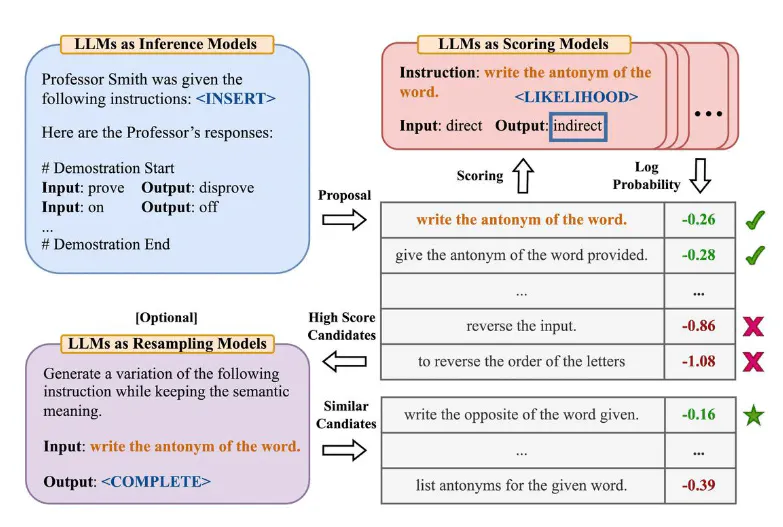
\includegraphics[width=\linewidth,keepaspectratio]{llm140}
\end{center}				

{\tiny (Ref: Applied LLMs Mastery 2024 - Aishwarya Reganti)}  
\end{frame}

%%%%%%%%%%%%%%%%%%%%%%%%%%%%%%%%%%%%%%%%%%%%%%%%%%%%%%%%%%%
\begin{frame}[fragile]\frametitle{LLM Pipeline Evaluation (2)}
  \begin{itemize}
    \item \textbf{Evaluating Prompts:}
      \begin{itemize}
        \item Evaluate prompts' impact on LLM output.
        \item Utilize prompt testing frameworks.
        \item Tools like Promptfoo, PromptLayer, etc., are commonly used.
      \end{itemize}
    \item \textbf{Automatic Prompt Generation:}
      \begin{itemize}
        \item Recent methods automate prompt optimization.
        \item Example: Automatic Prompt EngineerAPE.
      \end{itemize}
  \end{itemize}
\end{frame}

%%%%%%%%%%%%%%%%%%%%%%%%%%%%%%%%%%%%%%%%%%%%%%%%%%%%%%%%%%%
\begin{frame}[fragile]\frametitle{LLM Pipeline Evaluation (3)}
  \begin{itemize}
    \item \textbf{Evaluating Retrieval Pipeline:}
      \begin{itemize}
        \item Essential for LLM pipelines, especially RAG use-cases.
        \item Assessing top-k retrieved documents' quality.
      \end{itemize}
    \item \textbf{Metrics for Context Quality:}
      \begin{itemize}
        \item Context Precision.
		$$\text{Context Precision@k} = {\sum {\text{precision@k}} \over \text{total number of relevant items in the top K results}}$$
        \item Context Relevancy. $$\text{context relevancy} = {|S| \over |\text{Total number of sentences in retrived context}|}$$
        \item Context Recall.
      \end{itemize}
  \end{itemize}

\end{frame}

%%%%%%%%%%%%%%%%%%%%%%%%%%%%%%%%%%%%%%%%%%%%%%%%%%%%%%%%%%%
\begin{frame}[fragile]\frametitle{LLM Pipeline Evaluation (3)}
  
\begin{lstlisting}
Hint

Question: What is the capital of France?

High context relevancy: France, in Western Europe, encompasses medieval cities, alpine villages and Mediterranean beaches. Paris, its capital, is famed for its fashion houses, classical art museums including the Louvre and monuments like the Eiffel Tower.

Low context relevancy: France, in Western Europe, encompasses medieval cities, alpine villages and Mediterranean beaches. Paris, its capital, is famed for its fashion houses, classical art museums including the Louvre and monuments like the Eiffel Tower. The country is also renowned for its wines and sophisticated cuisine. Lascaux’s ancient cave drawings, Lyon’s Roman theater and the vast Palace of Versailles attest to its rich history.

\end{lstlisting}  
			

\end{frame}

%%%%%%%%%%%%%%%%%%%%%%%%%%%%%%%%%%%%%%%%%%%%%%%%%%%%%%%%%%%
\begin{frame}[fragile]\frametitle{LLM Pipeline Evaluation (4)}
  \begin{itemize}
    \item \textbf{Metrics for Context Quality (contd.):}
      \begin{itemize}
        \item Mean Average Precision (MAP).
        \item Normalized Discounted Cumulative Gain (nDCG).
        \item Reciprocal Rank.
        \item Mean Reciprocal Rank (MRR).
      \end{itemize}
  \end{itemize}
\end{frame}


%%%%%%%%%%%%%%%%%%%%%%%%%%%%%%%%%%%%%%%%%%%%%%%%%%%%%%%%%%%
\begin{frame}[fragile]\frametitle{LLM Model Evaluation (1)}
  \begin{itemize}
    \item \textbf{Introduction:}
      \begin{itemize}
        \item Assessing the core of the pipeline: the LLM model.
        \item Evaluation complexity arises due to broad applicability.
      \end{itemize}
  \end{itemize}
\end{frame}

%%%%%%%%%%%%%%%%%%%%%%%%%%%%%%%%%%%%%%%%%%%%%%%%%%%%%%%%%%%
\begin{frame}[fragile]\frametitle{LLM Model Evaluation (2)}
  \begin{itemize}
    \item \textbf{Dimensions of LLM Evaluation:}
      \begin{itemize}
        \item Relevance Metrics.
        \item Alignment Metrics.
        \item Task-Specific Metrics.
      \end{itemize}
  \end{itemize}
\end{frame}

%%%%%%%%%%%%%%%%%%%%%%%%%%%%%%%%%%%%%%%%%%%%%%%%%%%%%%%%%%%
\begin{frame}[fragile]\frametitle{LLM Model Evaluation (3)}
  \begin{itemize}
    \item \textbf{Relevance Metrics:}
      \begin{itemize}
        \item Assess pertinence of response to user's query and context.
      \end{itemize}
    \item \textbf{Alignment Metrics:}
      \begin{itemize}
        \item Evaluate alignment with human preferences.
        \item Consider fairness, robustness, and privacy.
      \end{itemize}
  \end{itemize}
\end{frame}

%%%%%%%%%%%%%%%%%%%%%%%%%%%%%%%%%%%%%%%%%%%%%%%%%%%%%%%%%%%
\begin{frame}[fragile]\frametitle{LLM Model Evaluation (4)}
  \begin{itemize}
    \item \textbf{Task-Specific Metrics:}
      \begin{itemize}
        \item Gauge LLM performance across various tasks.
        \item Examples: multihop reasoning, mathematical reasoning, etc.
      \end{itemize}
  \end{itemize}
\end{frame}

%%%%%%%%%%%%%%%%%%%%%%%%%%%%%%%%%%%%%%%%%%%%%%%%%%%%%%%%%%%
\begin{frame}[fragile]\frametitle{Relevance Metrics (1)}
  \begin{itemize}
    \item \textbf{Introduction:}
      \begin{itemize}
        \item Evaluation metrics focusing on response relevance.
      \end{itemize}
  \end{itemize}
\end{frame}

%%%%%%%%%%%%%%%%%%%%%%%%%%%%%%%%%%%%%%%%%%%%%%%%%%%%%%%%%%%
\begin{frame}[fragile]\frametitle{Relevance Metrics (2)}
  \begin{itemize}
    \item \textbf{Common Metrics:}
      \begin{itemize}
        \item \textbf{Perplexity:} Measures text prediction quality. Lower values indicate better performance.
        \item \textbf{Human Evaluation:} Human assessors judge relevance, fluency, coherence, and overall quality.
        \item \textbf{BLEU (Bilingual Evaluation Understudy):} Compares generated output with a reference answer. Higher scores indicate better performance.
      \end{itemize}
  \end{itemize}
\end{frame}

%%%%%%%%%%%%%%%%%%%%%%%%%%%%%%%%%%%%%%%%%%%%%%%%%%%%%%%%%%%
\begin{frame}[fragile]\frametitle{Relevance Metrics (3)}
  \begin{itemize}
    \item \textbf{Diversity Metric:}
      \begin{itemize}
        \item Measures variety and uniqueness of LLM responses.
        \item Includes n-gram diversity or semantic similarity metrics.
        \item Higher scores indicate more diverse and unique outputs.
      \end{itemize}
  \end{itemize}
\end{frame}

%%%%%%%%%%%%%%%%%%%%%%%%%%%%%%%%%%%%%%%%%%%%%%%%%%%%%%%%%%%
\begin{frame}[fragile]\frametitle{Relevance Metrics (4)}
  \begin{itemize}
    \item \textbf{ROUGE (Recall-Oriented Understudy for Gisting Evaluation):}
      \begin{itemize}
        \item Evaluates LLM-generated text quality by comparing it with reference text.
        \item Assesses precision, recall, and F1-score.
        \item Provides insights into similarity between generated and reference texts.
      \end{itemize}
  \end{itemize}
\end{frame}

%%%%%%%%%%%%%%%%%%%%%%%%%%%%%%%%%%%%%%%%%%%%%%%%%%%%%%%%%%%
\begin{frame}[fragile]\frametitle{RAG Specific Relevance Metrics (1)}
  \begin{itemize}
    \item \textbf{Introduction:}
      \begin{itemize}
        \item RAG pipelines employ specific relevance metrics beyond generic ones.
      \end{itemize}
    \item \textbf{Faithfulness (From RAGas Documentation):}
      \begin{itemize}
        \item Measures factual consistency of the generated answer against the provided context.
        \item Calculated from answer and retrieved context, scaled to (0,1) range.
        \item Higher score indicates better faithfulness.
      \end{itemize}
  \end{itemize}
\end{frame}

%%%%%%%%%%%%%%%%%%%%%%%%%%%%%%%%%%%%%%%%%%%%%%%%%%%%%%%%%%%
\begin{frame}[fragile]\frametitle{RAG Specific Relevance Metrics (3)}
  \begin{itemize}
    \item \textbf{Faithfulness Calculation:}
      \begin{itemize}
        \item Identify claims in the generated answer.
        \item Cross-check each claim with the given context for inference.
        \item Faithfulness score is based on the ability to infer claims from context.
      \end{itemize}
  \end{itemize}
$${|\text{Number of claims in the generated answer that can be inferred from given context}| \over |\text{Total number of claims in the generated answer}|}$$  

\begin{lstlisting}
Hint

Question: Where and when was Einstein born?

Context: Albert Einstein (born 14 March 1879) was a German-born theoretical physicist, widely held to be one of the greatest and most influential scientists of all time

High faithfulness answer: Einstein was born in Germany on 14th March 1879.

Low faithfulness answer: Einstein was born in Germany on 20th March 1879.
\end{lstlisting}
\end{frame}

%%%%%%%%%%%%%%%%%%%%%%%%%%%%%%%%%%%%%%%%%%%%%%%%%%%%%%%%%%%
\begin{frame}[fragile]\frametitle{RAG Specific Relevance Metrics (4)}
  \begin{itemize}
    \item \textbf{Answer Relevance (From RAGas Documentation):}
      \begin{itemize}
        \item Focuses on assessing how pertinent the generated answer is to the given prompt.
        \item Scores between 0 and 1, where higher scores indicate better relevancy.
        \item Emphasizes completeness and avoids redundancy in answers.
      \end{itemize}
  \end{itemize}
\end{frame}

%%%%%%%%%%%%%%%%%%%%%%%%%%%%%%%%%%%%%%%%%%%%%%%%%%%%%%%%%%%
\begin{frame}[fragile]\frametitle{RAG Specific Relevance Metrics (5)}
  \begin{itemize}
    \item \textbf{Assessment Criteria:}
      \begin{itemize}
        \item Relevance based on how well the answer addresses the original question.
        \item Importance given to completeness, penalizing incomplete or redundant answers.
        \item Evaluation does not directly consider factuality.
      \end{itemize}
  \end{itemize}
\end{frame}

%%%%%%%%%%%%%%%%%%%%%%%%%%%%%%%%%%%%%%%%%%%%%%%%%%%%%%%%%%%
\begin{frame}[fragile]\frametitle{RAG Specific Relevance Metrics (6)}
  \begin{itemize}
    \item \textbf{Scoring Process:}
      \begin{itemize}
        \item LLM prompted to generate an appropriate question for the answer multiple times.
        \item Mean cosine similarity between generated questions and the original question is measured.
        \item Higher scores indicate better alignment between generated answer and the original question.
      \end{itemize}
  \end{itemize}
\end{frame}

%%%%%%%%%%%%%%%%%%%%%%%%%%%%%%%%%%%%%%%%%%%%%%%%%%%%%%%%%%%
\begin{frame}[fragile]\frametitle{RAG Specific Relevance Metrics (7)}
  \begin{itemize}
    \item \textbf{Answer Semantic Similarity (From RAGas Documentation):}
      \begin{itemize}
        \item Assesses semantic resemblance between the generated answer and the ground truth.
        \item Values range from 0 to 1, with higher scores indicating better alignment.
        \item Utilizes a cross-encoder model for calculating semantic similarity.
      \end{itemize}
  \end{itemize}
\end{frame}

%%%%%%%%%%%%%%%%%%%%%%%%%%%%%%%%%%%%%%%%%%%%%%%%%%%%%%%%%%%
\begin{frame}[fragile]\frametitle{Alignment Metrics in LLMs (1)}
  \begin{itemize}
    \item \textbf{Importance of Alignment Metrics:}
      \begin{itemize}
        \item Crucial, especially in applications directly interacting with people.
        \item Ensures conformity to acceptable human standards.
        \item Difficulty in mathematical quantification; relies on specific tests and benchmarks.
      \end{itemize}
  \end{itemize}
\end{frame}

%%%%%%%%%%%%%%%%%%%%%%%%%%%%%%%%%%%%%%%%%%%%%%%%%%%%%%%%%%%
\begin{frame}[fragile]\frametitle{Alignment Metrics in LLMs (2)}
  \begin{itemize}
    \item \textbf{Evaluation Challenge:}
      \begin{itemize}
        \item Difficult to quantify alignment metrics mathematically.
        \item Adoption of indirect measures through tests on specialized benchmarks.
        \item No universally correct method for evaluation.
      \end{itemize}
  \end{itemize}
\end{frame}

%%%%%%%%%%%%%%%%%%%%%%%%%%%%%%%%%%%%%%%%%%%%%%%%%%%%%%%%%%%
\begin{frame}[fragile]\frametitle{Alignment Dimensions (3)}
  \begin{itemize}
    \item \textbf{Dimensions for Alignment Evaluation:}
      \begin{itemize}
        \item Truthfulness: Accurate representation of information.
        \item Safety: Avoidance of unsafe or illegal outputs, promotion of healthy conversations.
        \item Fairness: Prevention of biased outcomes, assessment of stereotypes and biases.
        \item Robustness: Stability and performance across various input conditions.
        \item Privacy: Preservation of human and data autonomy, evaluation of privacy awareness.
      \end{itemize}
  \end{itemize}
\end{frame}

%%%%%%%%%%%%%%%%%%%%%%%%%%%%%%%%%%%%%%%%%%%%%%%%%%%%%%%%%%%
\begin{frame}[fragile]\frametitle{Alignment Dimensions (4)}
  \begin{itemize}
    \item \textbf{More Alignment Dimensions:}
      \begin{itemize}
        \item Machine Ethics: Challenges in defining machine ethics, divided into implicit ethics, explicit ethics, and emotional awareness.
        \item Transparency: Concerns the availability of information about LLMs and their outputs.
        \item Accountability: Ability to autonomously provide explanations for behavior.
        \item Regulations and Laws: Abiding by rules and regulations posed by nations and organizations.
      \end{itemize}
  \end{itemize}
\end{frame}

%%%%%%%%%%%%%%%%%%%%%%%%%%%%%%%%%%%%%%%%%%%%%%%%%%%%%%%%%%%
\begin{frame}[fragile]\frametitle{Dissection of Dimensions (5)}
  \begin{itemize}
    \item \textbf{Detailed Analysis:}
      \begin{itemize}
        \item Each dimension further dissected into specific categories.
        \item Example: Truthfulness segmented into misinformation, hallucination, sycophancy, and adversarial factuality.
        \item Corresponding datasets and metrics designed for quantification.
      \end{itemize}
  \end{itemize}
\end{frame}


%%%%%%%%%%%%%%%%%%%%%%%%%%%%%%%%%%%%%%%%%%%%%%%%%%%%%%%%%%%
\begin{frame}[fragile]\frametitle{Key Characteristics}
  \begin{itemize}
    \item Quantitative: Metrics should provide a numerical score for task evaluation.
    \item Set a minimum passing threshold for determining LLM application adequacy.
    \item Monitor score changes over time to iterate and improve implementation.
    \item Reliable: Ensure consistency in metric performance, especially with unpredictable LLM outputs.
    \item Beware of inconsistency in LLM-Evals like G-Eval; traditional scoring methods may be more stable.
    \item Accurate: Align metrics with human expectations for meaningful evaluation.
    \item Reliable scores are meaningless if they do not truly reflect LLM application performance.
  \end{itemize}
\end{frame}

%%%%%%%%%%%%%%%%%%%%%%%%%%%%%%%%%%%%%%%%%%%%%%%%%%%%%%%%%%%
\begin{frame}[fragile]\frametitle{Achieving Reliability and Accuracy}
  \begin{itemize}
    \item The challenge: LLM outputs can be unpredictable.
    \item LLM-Evals often fall short in consistency.
    \item How can LLM evaluation metrics compute reliable and accurate scores?
  \end{itemize}
\end{frame}


%%%%%%%%%%%%%%%%%%%%%%%%%%%%%%%%%%%%%%%%%%%%%%%%%%%%%%%%%%%
\begin{frame}[fragile]\frametitle{Different Ways to Compute Metric Scores}


\begin{center}
\includegraphics[width=\linewidth,keepaspectratio]{llm_eval2}
\end{center}		
		
{\tiny (Ref: LLM Evaluation Metrics: Everything You Need for LLM Evaluation - Jeffrey Ip}
			
			
\end{frame}


%%%%%%%%%%%%%%%%%%%%%%%%%%%%%%%%%%%%%%%%%%%%%%%%%%%%%%%%%%%
\begin{frame}[fragile]\frametitle{Introduction to Statistical Scorers}
  \begin{itemize}
    \item Statistical scoring methods are often considered non-essential for LLM evaluation.
    \item If time is a constraint, feel free to skip to the "G-Eval" section.
    \item Statistical methods perform poorly in reasoning tasks, making them inaccurate for many LLM evaluation criteria.
  \end{itemize}
\end{frame}

%%%%%%%%%%%%%%%%%%%%%%%%%%%%%%%%%%%%%%%%%%%%%%%%%%%%%%%%%%%
\begin{frame}[fragile]\frametitle{Overview of Statistical Scorers}
  \begin{itemize}
    \item BLEU Scorer:
      \begin{itemize}
        \item Evaluates LLM output against annotated ground truths.
        \item Calculates precision for matching n-grams, applying brevity penalty if needed.
      \end{itemize}
    \item ROUGE Scorer:
      \begin{itemize}
        \item Primarily used for text summary evaluation in NLP models.
        \item Calculates recall through n-gram overlap between LLM output and expected output.
      \end{itemize}
    \item METEOR Scorer:
      \begin{itemize}
        \item Comprehensive metric assessing precision and recall, accounting for word order differences.
        \item Utilizes external linguistic databases like WordNet for synonyms.
      \end{itemize}
    \item Levenshtein Distance Scorer:
      \begin{itemize}
        \item Calculates minimum edits required for word or text string transformation.
        \item Useful for tasks like spelling corrections with critical character alignment.
      \end{itemize}
  \end{itemize}
\end{frame}

%%%%%%%%%%%%%%%%%%%%%%%%%%%%%%%%%%%%%%%%%%%%%%%%%%%%%%%%%%%
\begin{frame}[fragile]\frametitle{Limitations of Statistical Scorers}
  \begin{itemize}
    \item Purely statistical scorers lack semantic consideration and have limited reasoning capabilities.
    \item Inaccuracy in evaluating long and complex LLM outputs.
  \end{itemize}
\end{frame}

%%%%%%%%%%%%%%%%%%%%%%%%%%%%%%%%%%%%%%%%%%%%%%%%%%%%%%%%%%%
\begin{frame}[fragile]\frametitle{Introduction to Model-Based Scorers}
  \begin{itemize}
    \item Purely statistical scorers are reliable but lack accuracy in semantics.
    \item Model-based scorers, relying on NLP models, are comparatively more accurate but less reliable due to their probabilistic nature.
  \end{itemize}
\end{frame}

%%%%%%%%%%%%%%%%%%%%%%%%%%%%%%%%%%%%%%%%%%%%%%%%%%%%%%%%%%%
\begin{frame}[fragile]\frametitle{Comparison with Non-LLM Scorers}
  \begin{itemize}
    \item Non-LLM scorers perform worse than LLM-Evals due to similar reasons as statistical scorers.
    \item Examples of non-LLM scorers:
      \begin{itemize}
        \item NLI Scorer:
          \begin{itemize}
            \item Uses Natural Language Inference models for logical consistency classification.
            \item Scores range between entailment (1) and contradiction (0).
          \end{itemize}
        \item BLEURT Scorer:
          \begin{itemize}
            \item Utilizes pre-trained models like BERT for scoring LLM outputs.
          \end{itemize}
      \end{itemize}
  \end{itemize}
\end{frame}

%%%%%%%%%%%%%%%%%%%%%%%%%%%%%%%%%%%%%%%%%%%%%%%%%%%%%%%%%%%
\begin{frame}[fragile]\frametitle{Shortcomings of Model-Based Scorers}
  \begin{itemize}
    \item Inconsistent scores are a common challenge.
    \item NLI scorers may struggle with accuracy on processing long texts.
    \item BLEURT is limited by the quality and representativeness of its training data.
  \end{itemize}
\end{frame}

%%%%%%%%%%%%%%%%%%%%%%%%%%%%%%%%%%%%%%%%%%%%%%%%%%%%%%%%%%%
\begin{frame}[fragile]\frametitle{G-Eval}

G-Eval is a recently developed framework from a paper titled ``NLG Evaluation using GPT-4 with Better Human Alignment'' that uses LLMs to evaluate LLM outputs (aka. LLM-Evals).

\begin{center}
\includegraphics[width=\linewidth,keepaspectratio]{llm_eval3}
\end{center}		
		
{\tiny (Ref: LLM Evaluation Metrics: Everything You Need for LLM Evaluation - Jeffrey Ip}
			
			
\end{frame}

%%%%%%%%%%%%%%%%%%%%%%%%%%%%%%%%%%%%%%%%%%%%%%%%%%%%%%%%%%%
\begin{frame}[fragile]\frametitle{Introduction to G-Eval}
  \begin{itemize}
    \item G-Eval generates evaluation steps using Chain of Thoughts (CoTs).
    \item Final score determined through a form-filling paradigm.
    \item Requires several pieces of information for evaluation.
    \item Evaluates LLM output coherence by constructing a prompt with criteria and text.
  \end{itemize}
\end{frame}

%%%%%%%%%%%%%%%%%%%%%%%%%%%%%%%%%%%%%%%%%%%%%%%%%%%%%%%%%%%
\begin{frame}[fragile]\frametitle{G-Eval Algorithm Steps}
  \begin{enumerate}
    \item Introduce evaluation task to LLM (e.g., rate coherence from 1-5).
    \item Define criteria (e.g., "Coherence - quality of all sentences").
    \item Concatenate evaluation steps and arguments to create a prompt.
    \item Ask LLM to generate a score between 1-5.
    \item (Optional) Normalize the score using probabilities of output tokens.
    \item Access to raw model embeddings is currently unavailable via the OpenAI API (as of 2024).
  \end{enumerate}
\end{frame}

%%%%%%%%%%%%%%%%%%%%%%%%%%%%%%%%%%%%%%%%%%%%%%%%%%%%%%%%%%%
\begin{frame}[fragile]\frametitle{Optional Normalization in G-Eval}
  \begin{itemize}
    \item Normalization step involves taking probabilities of output tokens.
    \item Calculate weighted summation for a more fine-grained result.
    \item Introduced in the paper to minimize bias in LLM scoring.
    \item Offers more detailed scores on a 1-5 scale.
  \end{itemize}
\end{frame}

%%%%%%%%%%%%%%%%%%%%%%%%%%%%%%%%%%%%%%%%%%%%%%%%%%%%%%%%%%%
\begin{frame}[fragile]\frametitle{G-Eval Metrics}


\begin{center}
\includegraphics[width=\linewidth,keepaspectratio]{llm_eval4}
\end{center}		
		
{\tiny (Ref: LLM Evaluation Metrics: Everything You Need for LLM Evaluation - Jeffrey Ip}
			
			
\end{frame}

%%%%%%%%%%%%%%%%%%%%%%%%%%%%%%%%%%%%%%%%%%%%%%%%%%%%%%%%%%%
\begin{frame}[fragile]\frametitle{Advantages of G-Eval}
  \begin{itemize}
    \item LLM-Eval that considers full semantics of LLM outputs.
    \item More accurate compared to non-LLM scorers.
    \item Non-LLM scorers lack the capability to understand the full scope of LLM-generated text.
  \end{itemize}
\end{frame}

%%%%%%%%%%%%%%%%%%%%%%%%%%%%%%%%%%%%%%%%%%%%%%%%%%%%%%%%%%%
\begin{frame}[fragile]\frametitle{Limitations of G-Eval}
  \begin{itemize}
    \item Although correlates more with human judgment, it can still be unreliable.
    \item Asking an LLM to produce a score is inherently arbitrary.
  \end{itemize}
\end{frame}


%%%%%%%%%%%%%%%%%%%%%%%%%%%%%%%%%%%%%%%%%%%%%%%%%%%%%%%%%%%
\begin{frame}[fragile]\frametitle{Considerations for Evaluation Metrics}
  \begin{itemize}
    \item Choice depends on the use case and LLM application architecture.
    \item RAG-based customer support chatbot on GPT models:
      \begin{itemize}
        \item Use RAG metrics (e.g., Faithfulness, Answer Relevancy, Contextual Precision).
      \end{itemize}
    \item Fine-tuning Mistral 7B:
      \begin{itemize}
        \item Utilize metrics like bias to ensure impartial LLM decisions.
      \end{itemize}
  \end{itemize}
\end{frame}


%%%%%%%%%%%%%%%%%%%%%%%%%%%%%%%%%%%%%%%%%%%%%%%%%%%%%%%%%%%
\begin{frame}[fragile]\frametitle{Introduction to RAG Metrics}
  \begin{itemize}
    \item RAG (Retrieval Augmented Generation) supplements LLMs for tailored outputs.
    \item Components: Retriever and Generator.
  \end{itemize}

RAG Workflow
  \begin{itemize}
    \item RAG system receives input.
    \item Retriever performs vector search in knowledge base (often a vector database).
    \item Generator uses retrieval context and user input to produce a tailored output.
  \end{itemize}

Key Insight in RAG Metrics
  \begin{itemize}
    \item High-quality LLM outputs result from a great retriever and generator.
    \item RAG metrics focus on evaluating retriever or generator reliably and accurately.
    \item Originally designed as reference-less metrics, usable even in a production setting.
  \end{itemize}
\end{frame}

%%%%%%%%%%%%%%%%%%%%%%%%%%%%%%%%%%%%%%%%%%%%%%%%%%%%%%%%%%%
\begin{frame}[fragile]\frametitle{Introduction to Faithfulness Metric}
  \begin{itemize}
    \item Faithfulness is an essential RAG metric.
    \item Evaluates if LLM/generator aligns factually with information in retrieval context.
  \end{itemize}
  
Choosing the Right Scorer
  \begin{itemize}
    \item QAG Scorer is the best for RAG metrics.
    \item Excels in tasks with a clear objective.
    \item For faithfulness, define it as the proportion of truthful claims in LLM output regarding retrieval context.
  \end{itemize}
\end{frame}

%%%%%%%%%%%%%%%%%%%%%%%%%%%%%%%%%%%%%%%%%%%%%%%%%%%%%%%%%%%
\begin{frame}[fragile]\frametitle{Calculating Faithfulness with QAG}
  \begin{enumerate}
    \item Use LLMs to extract all claims in the output.
    \item For each claim, check agreement or contradiction with each individual node in the retrieval context.
    \item QAG close-ended question: "Does the claim agree with the reference text?"
    \item Answer options: 'yes,' 'no,' or 'idk' (no relevant information).
    \item Total truthful claims: sum of 'yes' and 'idk.'
    \item Divide by the total number of claims made.
  \end{enumerate}
\end{frame}

%%%%%%%%%%%%%%%%%%%%%%%%%%%%%%%%%%%%%%%%%%%%%%%%%%%%%%%%%%%
\begin{frame}[fragile]\frametitle{Advantages of QAG for Faithfulness}
  \begin{itemize}
    \item Utilizes LLM's advanced reasoning capabilities.
    \item Avoids unreliability in LLM-generated scores.
    \item Superior to G-Eval in terms of accuracy.
  \end{itemize}
\end{frame}

%%%%%%%%%%%%%%%%%%%%%%%%%%%%%%%%%%%%%%%%%%%%%%%%%%%%%%%%%%%
\begin{frame}[fragile]\frametitle{Introduction to Answer Relevancy Metric}
  \begin{itemize}
    \item Answer Relevancy: Crucial RAG metric.
    \item Assesses if RAG generator produces concise answers.
    \item Calculation: Proportion of relevant sentences in LLM output to total sentences.
  \end{itemize}
  
Building a Robust Answer Relevancy Metric
  \begin{itemize}
    \item Take retrieval context into account.
    \item Additional context may justify seemingly irrelevant sentence's relevancy.
  \end{itemize}
\end{frame}

%%%%%%%%%%%%%%%%%%%%%%%%%%%%%%%%%%%%%%%%%%%%%%%%%%%%%%%%%%%
\begin{frame}[fragile]\frametitle{Introduction to Contextual Precision}
  \begin{itemize}
    \item Contextual Precision: Crucial RAG metric.
    \item Evaluates quality of RAG pipeline's retriever.
    \item Concerned with the relevancy of retrieval context.
  \end{itemize}
Key Aspects of Contextual Precision
  \begin{itemize}
    \item High contextual precision scores prioritize relevant nodes in retrieval context.
    \item Ranking relevant nodes higher than irrelevant ones is crucial.
    \item LLMs assign more weight to information in nodes appearing earlier in retrieval context.
    \item Influences the quality of the final output.
  \end{itemize}
\end{frame}

%%%%%%%%%%%%%%%%%%%%%%%%%%%%%%%%%%%%%%%%%%%%%%%%%%%%%%%%%%%
\begin{frame}[fragile]\frametitle{Introduction to Contextual Recall}
  \begin{itemize}
    \item Contextual Recall: Additional metric for RAG evaluation.
    \item Calculates proportion of relevant sentences in expected output attributed to retrieval context nodes.
    \item Higher score indicates better alignment between retrieved information and expected output.
  \end{itemize}
Calculating Contextual Recall
  \begin{itemize}
    \item Proportion of sentences in expected output related to retrieval context nodes.
    \item Indicates retriever's effectiveness in sourcing relevant and accurate content.
    \item Aids the generator in producing contextually appropriate responses.
  \end{itemize}
\end{frame}

%%%%%%%%%%%%%%%%%%%%%%%%%%%%%%%%%%%%%%%%%%%%%%%%%%%%%%%%%%%
\begin{frame}[fragile]\frametitle{Contextual Relevancy Metric}
  \begin{itemize}
    \item Simplest metric: Proportion of relevant sentences in retrieval context to a given input.
  \end{itemize}
\end{frame}

%%%%%%%%%%%%%%%%%%%%%%%%%%%%%%%%%%%%%%%%%%%%%%%%%%%%%%%%%%%
\begin{frame}[fragile]\frametitle{Fine-Tuning Metrics Overview}
  \begin{itemize}
    \item Assess LLM itself, not the entire system.
    \item Commonly fine-tuned for:
      \begin{itemize}
        \item Incorporating additional contextual knowledge.
        \item Adjusting behavior.
      \end{itemize}
  \end{itemize}
\end{frame}

%%%%%%%%%%%%%%%%%%%%%%%%%%%%%%%%%%%%%%%%%%%%%%%%%%%%%%%%%%%
\begin{frame}[fragile]\frametitle{Hallucination Metric}
  \begin{itemize}
    \item Similar to faithfulness but more complex.
    \item Difficult to pinpoint exact ground truth for output.
    \item SelfCheckGPT's zero-shot approach can sample proportion of hallucinated sentences.
    \item Expensive approach; suggest using NLI scorer with manual context as ground truth.
  \end{itemize}
\end{frame}

%%%%%%%%%%%%%%%%%%%%%%%%%%%%%%%%%%%%%%%%%%%%%%%%%%%%%%%%%%%
\begin{frame}[fragile]\frametitle{Toxicity Metric}
  \begin{itemize}
    \item Evaluates offensive, harmful, or inappropriate language.
    \item Utilize pre-trained models like Detoxify with BERT scorer.
    \item Can be inaccurate due to association of certain words with toxicity.
  \end{itemize}
\end{frame}

%%%%%%%%%%%%%%%%%%%%%%%%%%%%%%%%%%%%%%%%%%%%%%%%%%%%%%%%%%%
\begin{frame}[fragile]\frametitle{Bias Metric}
  \begin{itemize}
    \item Evaluates political, gender, and social biases in textual content.
    \item Crucial for decision-making applications (e.g., bank loan approvals, recruitment).
    \item Assess with G-Eval or QAG (toxicity and bias).
    \item Highly subjective, varies across different environments.
    \item Implementation challenging; fine-tuning custom LLM could be a solution.
  \end{itemize}
\end{frame}

%%%%%%%%%%%%%%%%%%%%%%%%%%%%%%%%%%%%%%%%%%%%%%%%%%%%%%%%%%%
\begin{frame}[fragile]\frametitle{Use Case: Summarization}
  \begin{itemize}
    \item Factual alignment and inclusion crucial in good summaries.
    \item Using QAG, calculate both scores for a final summarization score.
    \item In DeepEval, final score is the minimum of the two intermediary scores.
  \end{itemize}
\end{frame}

%%%%%%%%%%%%%%%%%%%%%%%%%%%%%%%%%%%%%%%%%%%%%%%%%%%%%%%%%%%
\begin{frame}[fragile]\frametitle{Conclusion}
  \begin{itemize}
    \item Explored a comprehensive list of scorers and metrics.
    \item Understand factors and choices for selecting LLM evaluation metrics.
  \end{itemize}
Objective of LLM Evaluation Metrics
  \begin{itemize}
    \item Quantify performance of LLM (application).
    \item Various scorers available, with some more accurate than others.
  \end{itemize}
\end{frame}

%%%%%%%%%%%%%%%%%%%%%%%%%%%%%%%%%%%%%%%%%%%%%%%%%%%%%%%%%%%
\begin{frame}[fragile]\frametitle{Scorers for LLM Evaluation}
  \begin{itemize}
    \item LLM-based scorers (G-Eval, Prometheus, SelfCheckGPT, QAG) are most accurate.
    \item High reasoning capabilities enhance accuracy.
    \item Caution needed to ensure reliability of scores.
  \end{itemize}
Metric Choice Dependence
  \begin{itemize}
    \item Metrics choice depends on use case and LLM application implementation.
    \item RAG and fine-tuning metrics are a solid starting point for LLM output evaluation.
  \end{itemize}
Use Case Specific Metrics
  \begin{itemize}
    \item For more specific use cases, consider G-Eval with few-shot prompting.
    \item Ensures the most accurate results tailored to your application.
  \end{itemize}
\end{frame}
